\documentclass[kindlepaper]{BHCexam4kindle}
\usepackage{lipsum}
\begin{document}
\printanswers % 我要打印答案
	\biaoti{2019真题}
	\fubiaoti{}
	\maketitle
	\begin{questions}
		\qs 当 $x \rightarrow 0$ 时,$x-\tan x$与$x^{k}$是同阶无穷小, 则 k $=$ \xx
		\onech{1}{2}{3}{4}
		\begin{solution}
			当 $x \rightarrow 0$ 时,$x-\tan x \sim-\frac{1}{3} x^{3}$, 因此选 C.
		\end{solution}

		\qs 设函数$f(x)=\left\{\begin{array}{ll}{x|x|,} & {x \leqslant 0} \\ {x \ln x,} & {x>0}\end{array}\right.$
			则 $x=0$ 是 $f(x)$ 的 \xx
			\twoch{可导点, 极值点}{不可导点, 极值点}{可导点, 非极值点}{不可导点, 非极值点}
			\begin{solution}
				$\lim _{x \rightarrow 0^{-}} x|x|=\lim _{x \rightarrow 0^{+}} x \ln x=f(0)=0$,
				, 因此 $f(x)$ 在$x=0$ 处连续. 且当$x \in \stackrel{\circ}{U}\left(x_{0}\right)$时,
				$f(x)<0=f(0)$, 因此 $x=0$是 $f(x)$的极大值点. 而极限$\lim _{x \rightarrow 0^{+}} \frac{f(x)-f(0)}{x}=\lim _{x \rightarrow 0^{+}} \ln x$
				不存在, 因此不可导, 选 B.
			\end{solution}

		\qs 设 $\mathcal{U}_{n}$ 是单调增加的有界数列, 则下列级数中收敛的是 \xx
		\twoch{$\sum_{n=1}^{\infty} \frac{u_{n}}{n}$}{$\sum_{n=1}^{\infty}(-1)^{n} \frac{1}{u_{n}}$}{$\sum_{n=1}^{\infty}\left(1-\frac{u_{n}}{u_{n+1}}\right)$}{$\sum_{n=1}^{\infty}\left(u_{n+1}^{2}-u_{n}^{2}\right)$}
		\begin{solution}
			正确答案选 D. 因为 $\mathcal{U}_{n}$  单调递增有界, 故极限$\lim _{n \rightarrow \infty} u_{n}=a$ 存在, D 选项级数的部分
			和数列收敛, 因此级数收敛. A 和 B 中只要$a \neq 0$就发散. C 中可取反例$u_{n}=-\frac{1}{n}$, 则$1-\frac{u_{n}}{u_{n+1}}=\frac{1}{n+1}$
			, 调和级数发散.
		\end{solution}

		\qs 设函数 $Q(x, y)=\frac{x}{y^{2}}$, 如果对上半平面 $(y>0)$ 内的任意有向光滑闭曲线 $C$ 都有$\oint_{C} P(x, y) \mathrm{d} x+Q(x, y) \mathrm{d} y=0$, 那么函数可取为\xx
		\twoch{$y-\frac{x^{2}}{y}$}{$\frac{1}{y}-\frac{x^{2}}{y^{2}}$}{$\frac{1}{x}-\frac{1}{y}$}{$x-\frac{1}{y}$}
		\begin{solution}
			由题意, 应当选择函数$P(x, y)$ 使得在整个上半平面上均有$\frac{\partial P}{\partial y}=\frac{\partial Q}{\partial x}=\frac{1}{y^{2}}$
			成立, 选D(注意 C 选项在 y 轴上偏导数不存在).
		\end{solution}

		\qs 设$A$是 3 阶实对称矩阵,$E$ 是 3 阶单位矩阵, 若$A^{2}+A=2 E$, 且$|A|=4$4, 则二次
		型 $\boldsymbol{x}^{\mathrm{T}} \boldsymbol{A} \boldsymbol{x}$ 的规范形为\xx
		\twoch{$y_{1}^{2}+y_{2}^{2}+y_{3}^{2}$}{$y_{1}^{2}+y_{2}^{2}-y_{3}^{2}$}{$y_{1}^{2}-y_{2}^{2}-y_{3}^{2}$}{$-y_{1}^{2}-y_{2}^{2}-y_{3}^{2}$}
		\begin{solution}
			由 $A^{2}+A=2 E$ 可知矩阵$A$的特征值$\lambda$满足$\lambda^{2}+\lambda=2$, 因此$\lambda=1$ 或 $\lambda=2$. 再由
			$|A|=4$可知 A 的特征值为 2, 2, 1. 因此二次型 $\boldsymbol{x}^{\mathrm{T}} \boldsymbol{A} \boldsymbol{x}$的正惯性指数为$1$ , 负惯性指数为$2$, 选 $C$.
		\end{solution}

		\qs 如图所示, 有 3 张平面两两相交, 交线相互平行, 它们的方程\\
		$a_{i 1} x+a_{i 1} y+a_{i 3} z=d_{i}(i=1,2,3)$\\
		组成的线性方程组的系数矩阵和增广矩阵分别为 $\boldsymbol{A}, \overline{\boldsymbol{A}}$, 则\xx
		\fourch{$r(\boldsymbol{A})=2, r(\overline{\boldsymbol{A}})=3$}
		{$r(\boldsymbol{A})=2, r(\overline{\boldsymbol{A}})=2$}
		{$r(\boldsymbol{A})=1, r(\overline{\boldsymbol{A}})=2$}
		{$r(\boldsymbol{A})=1, r(\overline{\boldsymbol{A}})=1$}
		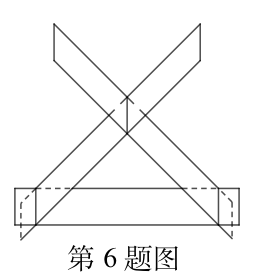
\includegraphics[width=2in]{img-2019/2019-06} 
		\begin{solution}
			令 $\boldsymbol{x}=(x, y, z)^{\mathrm{T}}, \boldsymbol{b}=\left(d_{1}, d_{2}, d_{3}\right)^{\mathrm{T}}$ , 由于三个平面无交点, 因此方程组$\boldsymbol{A x}=\boldsymbol{b}$$\boldsymbol{A x}=\boldsymbol{b}$ 无解.
		即 $r(\boldsymbol{A})<r(\overline{A}) \leqslant 3$. 再根据任意两个平面都不重合或平行, 可知 $A$ 的任意两行线性无关,
		因此 $r(\boldsymbol{A}) \geqslant 2$. 因此只能是$r(\boldsymbol{A})=2, r(\overline{A})=3$, 选 A.
		\end{solution}

		\qs 设 $A, B$ 为随机事件, 则 $P(A)=P(B)$ 的充分必要条件是\xx
		\fourch{$P(A \cup B)=P(A)+P(B)$}{$P(A B)=P(A) P(B)$}{$P(A \overline{B})=P(B \overline{A})$}{$P(A B)=P(\overline{A B})$}
		\begin{solution}
			显然 $P(A)=P(B)$等价于$P(A)-P(A B)=P(B)-P(A B)$, 即$P(A \overline{B})=P(B \overline{A})$,
			选 $C$. 对于选项 $A$ 和 $D$, 取 $A=B=\Omega$ 可排除; 对于选项 $B$, 取$B=\overline{A}$ 即可排除.
		\end{solution}

		\qs 设随机变量 $X$ 与 $Y$相互独立, 且都服从正态分布 $N\left(\mu, \sigma^{2}\right)$, 则$P\{|X-Y|<1\}$\xx
		\fourch{与$\mu$无关, 而与$\sigma^{2}$ 有关}
		{与$\mu$ 有关, 而与 $\sigma^{2}$ 无关}
		{与$\mu$, $\sigma^{2}$都有关}
		{与 $\mu$, $\sigma^{2}$ 都无关}
		\begin{solution}
			显然$P(A)=P(B)$等价于$P(A)-P(A B)=P(B)-P(A B)$,即$P(A \overline{B})=P(B \overline{A})$,
			选$C$,对于选项 $A$ 和 $D$, 取$A=B=\Omega$ 可排除; 对于选项 $B$, 取$B=\overline{A}$ 即可排除.
		\end{solution}

		\qs 由条件可知 $X-Y \sim N\left(0,2 \sigma^{2}\right)$, 因此\\
	$\begin{aligned} P\{|X-Y|<1\} &=P\left\{\left|\frac{X-Y}{\sqrt{2} \sigma}\right|<\frac{1}{\sqrt{2} \sigma}\right\} 
	\\ &=\Phi\left(\frac{1}{\sqrt{2} \sigma}\right)-\Phi\left(-\frac{1}{\sqrt{2} \sigma}\right)
	\\ &=2 \Phi\left(\frac{1}{\sqrt{2} \sigma}\right)-1 \end{aligned}$
		,此概率与 $\mu$ 无关, 与$\sigma^{2}$有关, 选 $A$.

		\qs 设函数$f(u)$ 可导,$z=f(\sin y-\sin x)+x y$, 则$\frac{1}{\cos x} \cdot \frac{\partial z}{\partial x}+\frac{1}{\cos y} \cdot \frac{\partial z}{\partial y}=$ \tk
		\begin{solution}
			首先$\frac{\partial z}{\partial x}=-\cos x f^{\prime}(\sin y-\sin x)+y, \frac{\partial z}{\partial y}=\cos y f^{\prime}(\sin y-\sin x)+x$,因此
			$\frac{1}{\cos x} \cdot \frac{\partial z}{\partial x}+\frac{1}{\cos y} \cdot \frac{\partial z}{\partial y}=\frac{y}{\cos x}+\frac{x}{\cos y}$.
		\end{solution}

		\qs 微分方程$2 y y^{\prime}-y^{2}-2=0$满足条件$y(0)=1$的特解$y=$\tk
		\begin{solution}
			方程变量分离可得$\frac{2 y}{y^{2}+2} \mathrm{d} y=\mathrm{d} x$,两边积分得$y^{2}+2=C \mathrm{e}^{x}$,
			由 $y(0)=1$ 可知$C=3$, 方程的解为$y=\sqrt{3 \mathrm{e}^{x}-2}$ (注意初值条件, 要舍去负的解).
		\end{solution} 

		\qs 幂级数$\sum_{n=0}^{\infty} \frac{(-1)^{n}}{(2 n) !} x^{n}$在 $(0,+\infty)$ 内的和函数$S(x)=$ \tk.
		\begin{solution}
			$\sum_{n=0}^{\infty} \frac{(-1)^{n}}{(2 n) !} x^{n}=\sum_{n=0}^{\infty} \frac{(-1)^{n}}{(2 n) !}(\sqrt{x})^{2 n}=\cos (\sqrt{x})$
		\end{solution}

		\qs 设 $\Sigma$ 为曲面 $x^{2}+y^{2}+4 z^{2}=4(z \geqslant 0)$的上侧, 则$\iint_{\Sigma} \sqrt{4-x^{2}-4 z^{2}} \mathrm{d} x \mathrm{d} y =$ \tk.
		\begin{solution}
			$\Sigma$ 在 $x O y$面的投影区域为$D=(x, y) | x^{2}+y^{2} \leqslant 4$, 因此\\
		$ \begin{aligned} \iint_{\Sigma} \sqrt{4-x^{2}-4 z^{2}} \mathrm{d} x \mathrm{d} y 
		\\=\iint_{D} \sqrt{4-x^{2}-\left(4-x^{2}-y^{2}\right)} \mathrm{d} x \mathrm{d} y 
		\\=\iint_{D}|y| \mathrm{d} x \mathrm{d} y=4 \int_{0}^{\frac{\pi}{2}} \mathrm{d} \theta \int_{0}^{2} r^{2} \sin \theta \mathrm{d} r=\frac{32}{3} 
		\end{aligned}$
		\end{solution}

		\qs 设$A=\left(\alpha_{1}, \alpha_{2}, \alpha_{3}\right)$为 3 阶矩阵, 若$\alpha_{1}, \alpha_{2}$ 线性无关, 且  
		$\alpha_{3}=-\alpha_{1}+2 \alpha_{2}$,则线性程组$A x=0$ 的通解为\tk
		\begin{solution}
			由条件可知$A$ 有且只有两个线性无关的列向量, 因此$r(A)=2$. 因为$\alpha_{3}=-\alpha_{1}+2 \alpha_{2}$,所以$A\left(\begin{array}{c}{1} \\ {-2} \\ {1}\end{array}\right)=\alpha_{1}-2 \alpha_{2}+\alpha_{3}=0$,
				, 因此$A x=0$的通解为$\boldsymbol{x}=k(1,-2,1)^{\mathrm{T}}, k \in \mathbb{R}$.
		\end{solution}

		\qs 设随机变量 $X$ 的概率密度为$f(x)=\left\{\begin{array}{ll}{\frac{x}{2},} & {0<x<2} \\ {0,} & {others}\end{array},$\\
			$ F(x)\right.$
			为 $X$ 的分布函数,$E(X)$ 为 $X$ 的数学期望, 则$P(F(X)>E(X)-1)=$\tk.
		\begin{solution}
			首先$E(X)=\int_{0}^{2} x \frac{x}{2} \mathrm{d} x=\frac{4}{3}$.再令$Y=F(X)$.则当$y \leqslant 0$时$P(Y \leqslant y)=0$;当
			$y \geqslant 1$时,$P(Y \leqslant y)=1$(注意分布函数$F(X)$的取值范围). 当$0<y<1$时,$P(Y \leqslant y )=P(F(X) \leqslant y)=P\left(X \leqslant F^{-1}(y)\right)=F\left(F^{-1}(y)\right)=y$.
			因此$Y=F(X) \sim U(0,1)$,
			$P(F(X)>E(X)-1)=P\left(Y>\frac{1}{3}\right)=\frac{2}{3}$.\\
			注:事实上我们在这里证明了一个很重要的结论: 如果$X$ 是一个连续型随机变量,
			$F(X)$ 是它的分布函数, 则随机变量$Y=F(X) \sim U(0,1)$
		\end{solution}

		\qs 设函数 $y(x)$是微分方程$y^{\prime}+x y=e^{-\frac{x^{2}}{2}}$
		满足条件$y(0)=0$的特解
		\begin{parts}
			\part 求$y(x)$.
			\part 求曲线 $y=y(x)$ 的凹凸区间及拐点.
		\end{parts}
		\begin{solution}
			\begin{parts}
			\part 由条件可得$\left(y \mathrm{e}^{\frac{1}{2} x^{2}}\right)^{\prime}=
			\mathrm{e}^{\frac{1}{2} x^{2}}\left(y^{\prime}+x y\right)=1$ 
			, 于是$y e^{\frac{1}{2} x^{2}}=x+C$ . 由 $y(0)=0$可知$C=0, y=x \mathrm{e}^{-\frac{1}{2} x^{2}}$.
			\part 计算可得$y^{\prime}=\mathrm{e}^{-\frac{1}{2} x^{2}}\left(1-x^{2}\right), 
			\\y^{\prime \prime}=\mathrm{e}^{-\frac{1}{2} x^{2}}\left(x^{3}-3 x\right)$,
			令 $y^{\prime \prime}=0$得$x=0, \pm \sqrt{3}$. 再根据二阶导数的符号可得凹区间为$(-\sqrt{3}, 0)$ 和 
			$(\sqrt{3},+\infty)$, 凸区间为$(-\infty,-\sqrt{3})$ 和$(0, \sqrt{3})$.\\拐点为$(0,0),\left(-\sqrt{3},-\sqrt{3} \mathrm{e}^{-\frac{3}{2}}\right),\left(\sqrt{3}, \sqrt{3} \mathrm{e}^{-\frac{3}{2}}\right)$
			\end{parts}
		\end{solution}

		\qs 设$a,b$为实数, 函数 $z=2+a x^{2}+b y^{2}$在点 $(3,4)$处的方向导数中,沿方向
		$l=-3 i-4 j$的方向导数最大, 最大值为 10.
		\begin{parts}
			\part 求 $a, b$;
			\part 求曲面$z=2+a x^{2}+b y^{2}(z \geqslant 0)$的面积.
		\end{parts}
		\begin{solution}
			\begin{parts}
				\part 多元函数在一点处方向导数的最大值是沿着梯度方向的方向导数, 且最大值等于梯度的模. 由条件可得
				$\operatorname{grad} z=(2 a x, 2 b y)$,于是$\operatorname{grad}\left.z\right|_{(3,4)}=(6 a, 8 b)$
				, 因此$\frac{6 a}{-3}=\frac{8 b}{-4}$且$a, b<0$, 解得 $a=b$. 再由$10=\sqrt{(6 a)^{2}+(8 b)^{2}}$可得$a=b=-1$
				\part 记曲面$z=2-x^{2}-y^{2}$在 $xOy$ 面的投影区域为$D : x^{2}+y^{2} \leqslant 2$, 则曲面的面积为\\
			$\begin{aligned} S &=\iint_{D} \sqrt{1+(-2 x)^{2}+(-2 y)^{2}} \mathrm{d} x \mathrm{d} y
			\\&=\iint_{D} \sqrt{1+4 x^{2}+4 y^{2}} \mathrm{d} x \mathrm{d} y 
			\\ &=\int_{0}^{2 \pi} \mathrm{d} \theta \int_{0}^{\sqrt{2}} \sqrt{1+4 r^{2}} r \mathrm{d} r
			=\frac{13}{3} \pi \end{aligned}$
			\end{parts}
		\end{solution}

		\qs 求曲线$y=\mathrm{e}^{-x} \sin x(x \geqslant 0)$与 x 轴之间图形的面积.
		\begin{solution}
			利用直角坐标系下的面积公式可得所求面积为\\
		$\begin{aligned} S &=\int_{0}^{+\infty} \mathrm{e}^{-x}|\sin x| \mathrm{d} x=\sum_{n=0}^{\infty} \int_{n \pi}^{(n+1) \pi} \mathrm{e}^{-x}|\sin x| \mathrm{d} x \\ &=\sum_{n=0}^{\infty} \int_{0}^{\pi} \mathrm{e}^{-(n \pi+t)}|\sin (n \pi+t)| \mathrm{d} t \\ &=\int_{0}^{\pi} \mathrm{e}^{-t} \sin t \mathrm{d} t \sum_{n=0}^{\infty} \mathrm{e}^{-n \pi} \\ &=\frac{1+\mathrm{e}^{-\pi}}{2} \cdot \frac{1}{1-\mathrm{e}^{-\pi}}=\frac{\mathrm{e}^{\pi}+1}{2\left(\mathrm{e}^{\pi}-1\right)} \end{aligned}$
			其中利用两次分部积分可得$\int_{0}^{\pi} \mathrm{e}^{-t} \sin x \mathrm{d} t=\frac{1+\mathrm{e}^{-\pi}}{2}$.
		\end{solution}

		\qs 设$a_{n}=\int_{0}^{1} x^{n} \sqrt{1-x^{2}} \mathrm{d} x(n=0,1,2, \cdots)$.
		\begin{parts}
			\part 证明: 数列$a_{n}$单调减少, 且$a_{n}=\frac{n-1}{n+2} a_{n-2}(n=2,3, \cdots)$;
			\part 求$\lim _{n \rightarrow \infty} \frac{a_{n}}{a_{n-1}}$.
		\end{parts}
		\begin{solution}
			\begin{parts}
				\part 当$0<x<1$时,$x^{n} \sqrt{1-x^{2}}>x^{n+1} \sqrt{1-x^{2}}$,因此由$a_{n}$的定义可知$a_{n}>a_{n+1}$,
				即数列$a_{n}$单调减少. 利用分部积分可得\\$a_{n} \\$
			$\begin{aligned} &=\int_{0}^{1} x^{n} \sqrt{1-x^{2}} \mathrm{d} x
			&=\frac{1}{n+1} \int_{0}^{1} \sqrt{1-x^{2}} \mathrm{d}\left(x^{n+1}\right) \\ &=\frac{1}{n+1} x^{n+1}\left.\sqrt{1-x^{2}}\right|_{0} ^{1}+\frac{1}{n+1} \int_{0}^{1} \frac{x^{n+2}}{\sqrt{1-x^{2}}} \mathrm{d} x \\ &=-\frac{1}{n+1} a_{n}-\frac{1}{n+1} \int_{0}^{1} \mathrm{d} \sqrt{1-x^{2}} \\ &=-\frac{1}{n+1} a_{n}+\frac{n-1}{n+1} a_{n-2} \end{aligned}$
				因此$\frac{n+2}{n+1} a_{n}=\frac{n-1}{n+1} a_{n-2}$,即$a_{n}=\frac{n-1}{n+2} a_{n-2}(n=2,3, \cdots)$.
				\part 由于$\frac{n-1}{n+2}<\frac{a_{n}}{a_{n-2}}<\frac{a_{n}}{a_{n-1}}<\frac{a_{n}}{a_{n}}=1$ ,
				由夹逼准则知$\lim _{n \rightarrow \infty} \frac{a_{n}}{a_{n-1}}=1$
			\end{parts}
		\end{solution}

		\qs 设$\Omega$是锥面$x^{2}+(y-z)^{2}=(1-z)^{2}(0 \leqslant z \leqslant 1)$与平面$z=0$围成的锥体, 求$\Omega$的形心坐标.
		\begin{solution}
			这题并不是一般的圆锥面,为此我们给
			出锥面的一般定义: 过定点 V 的动直线
			L 沿着一条确定的曲线$\Gamma$移动所形成的
			曲面 S 叫做锥面. 直线 L 称为 S 的母线,
			曲线 $\Gamma$称为 S 的准线, 而定点 V 则是 S
			的顶点. 在本题中, 锥面与 $xOy$ 面的交线
			$x^{2}+y^{2}=1, z=0$就是母线, 顶点则是
			$(0,1,1)$, 如右图. 此锥面在 $xOy$ 面的投影
			区域就是 $D=\left\{(x, y) | x^{2}+y^{2} \leqslant 1\right\}$, 因此
			这题我们采用切片法 (先二后一) 计算.\\
			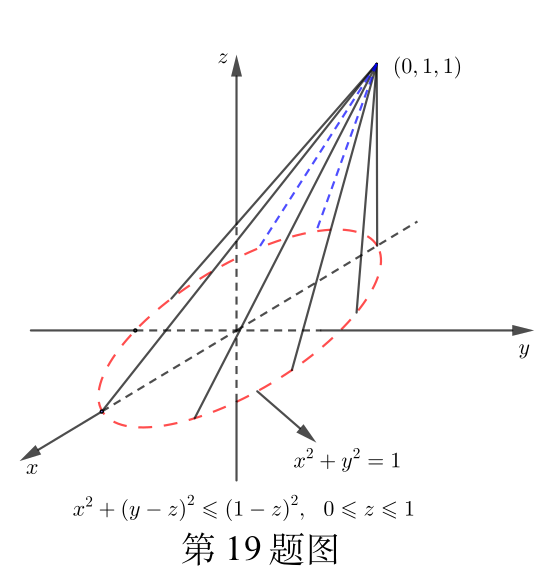
\includegraphics[width=2.7in]{img-2019/2019-19} 
			\\
			设形心坐标为$(\overline{x}, \overline{y}, \overline{z})$,由于$\Omega$是关于 $yOz$ 面对称的, 由对称性可知$\overline{x}=0$. 
			对固定的 $z$, 记$D_{z}=(x, y) | x^{2}+(y-z)^{2} \leqslant(1-z)^{2}$, 利用切片法可得\\
			$\iiint_{\Omega} \mathrm{d} V=\int_{0}^{1} \mathrm{d} z \iint_{D_{z}} \mathrm{d} x \mathrm{d} y=\pi \int_{0}^{1}(1-z)^{2} \mathrm{d} z=\frac{\pi}{3}$
$\iiint_{\Omega} z \mathrm{d} V=\int_{0}^{1} \mathrm{d} z \iint_{D_{z}} z \mathrm{d} x \mathrm{d} y=\pi \int_{0}^{1} z(1-z)^{2} \mathrm{d} z=\frac{\pi}{12}$
$\iiint_{\Omega} y \mathrm{d} V=\int_{0}^{1} \mathrm{d} z \iint_{D_{z}} y \mathrm{d} x \mathrm{d} y=\pi \int_{0}^{1} z(1-z)^{2} \mathrm{d} z=\frac{\pi}{12}$
			\\其中积分$\iint_{D_{z}} y \mathrm{d} x \mathrm{d} y$中, 令$y-z=u, \mathrm{d} y=\mathrm{d} u$, 则\\
			$\iint_{D_{z}} y \mathrm{d} x \mathrm{d} y=\iint_{x^{2}+u^{2} \leqslant(1-z)^{2}}(u+z) \mathrm{d} x \mathrm{u}=\pi z(1-z)^{2}$\\
			因此利用形心坐标公式得$\overline{y}=\overline{z}=\frac{\pi / 12}{\pi / 3}=\frac{1}{4}$, 形心坐标为$\left(0, \frac{1}{4}, \frac{1}{4}\right)$.
		\end{solution}

		\qs 设向量组$\boldsymbol{\alpha}_{1}=(1,2,1)^{\mathrm{T}}, \boldsymbol{\alpha}_{2}=(1,3,2)^{\mathrm{T}}, \boldsymbol{\alpha}_{3}=(1, a, 3)^{\mathrm{T}}$
		为$\mathbb{R}^{3}$的一组基,$\boldsymbol{\beta}=(1,1,1)^{\mathrm{T}}$在这组基下的坐标为$(b, c, 1)^{\mathrm{T}}$.
		\begin{parts}
			\part 求a,b,c;
			\part 证明:$\alpha_{2}, \alpha_{3}, \beta$为 $\mathbb{R}^{3}$ 的一组基, 并求 $\alpha_{2}, \alpha_{3}, \beta$ 
			到 $\alpha_{1}, \alpha_{2}, \alpha_{3}$ 的过渡矩阵.
		\end{parts}
		\begin{solution}
			\begin{parts}
			\part 由题意可知$b \boldsymbol{\alpha}_{1}+c \boldsymbol{\alpha}_{2}+\boldsymbol{\alpha}_{3}=\boldsymbol{\beta}$, 即\\
		$\left\{\begin{array}{l}{b+c+1=1} \\ {2 b+3 c+a=1} \\ {b+2 c+3=1}\end{array}\right.$,
			解得$a=3, b=2, c=-2$.
			\part 由于$\left|\alpha_{2}, \alpha_{3}, \beta\right|=\left|\begin{array}{ccc}{1} & {1} & {1} \\ {3} & {3} & {1} \\ {2} & {3} & {1}\end{array}\right|=\left|\begin{array}{ccc}{1} & {1} & {1} \\ {0} & {0} & {-2} \\ {0} & {1} & {-1}\end{array}\right|=2 \neq 0$
				,因此$r\left(\boldsymbol{\alpha}_{2}, \boldsymbol{\alpha}_{2}, \boldsymbol{\beta}\right)=3$,
				这说明$\alpha_{2}, \alpha_{3}, \beta$是$\mathbb{R}^{3}$的一组基.再由\\
			$\left(\boldsymbol{\alpha}_{2}, \boldsymbol{\alpha}_{3}, \boldsymbol{\beta}\right)=\left(\boldsymbol{\alpha}_{2}, \boldsymbol{\alpha}_{3}, 2 \boldsymbol{\alpha}_{1}-2 \boldsymbol{\alpha}_{2}+\boldsymbol{\alpha}_{3}\right)=\left(\boldsymbol{\alpha}_{1}, \boldsymbol{\alpha}_{2}, \boldsymbol{\alpha}_{3}\right)\left(\begin{array}{ccc}{0} & {0} & {2} \\ {1} & {0} & {-2} \\ {0} & {1} & {1}\end{array}\right)$\\
				可得\\
			$\left(\boldsymbol{\alpha}_{1}, \boldsymbol{\alpha}_{2}, \boldsymbol{\alpha}_{3}\right)=\left(\boldsymbol{\alpha}_{2}, \boldsymbol{\alpha}_{3}, \boldsymbol{\beta}\right)\left(\begin{array}{ccc}{0} & {0} & {2} \\ {1} & {0} & {-2} \\ {0} & {1} & {1}\end{array}\right)^{-1}=\left(\boldsymbol{\alpha}_{2}, \boldsymbol{\alpha}_{3}, \boldsymbol{\beta}\right)\left(\begin{array}{ccc}{1} & {1} & {0} \\ {-1 / 2} & {0} & {1} \\ {1 / 2} & {0} & {0}\end{array}\right)$,
					所以$\alpha_{2}, \alpha_{3}, \beta$到$\alpha_{1}, \alpha_{2}, \alpha_{3}$的过渡矩阵为$\left(\begin{array}{ccc}{1} & {1} & {0} \\ {-1 / 2} & {0} & {1} \\ {1 / 2} & {0} & {0}\end{array}\right)$.
			\end{parts}
		\end{solution}

		\qs 已知矩阵$A=\left(\begin{array}{ccc}{-2} & {-2} & {1} \\ {2} & {x} & {-2} \\ {0} & {0} & {-2}\end{array}\right)$
			与$\boldsymbol{B}=\left(\begin{array}{ccc}{2} & {1} & {0} \\ {0} & {-1} & {0} \\ {0} & {0} & {y}\end{array}\right)$
			相似.
		\begin{parts}
			\part 求 x,y;
			\part 求可逆矩阵 $P$ 使得$\boldsymbol{P}^{-1} \boldsymbol{A} \boldsymbol{P}=\boldsymbol{B}$.
		\end{parts}
		\begin{solution}
			\begin{parts}
				\part 由相似矩阵的性质可得\\
			$\left\{\begin{array}{l}{|A|=|\boldsymbol{B}|} \\ {\operatorname{tr}(\boldsymbol{A})=\operatorname{tr}(\boldsymbol{B})}\end{array} \Rightarrow\left\{\begin{array}{l}{4 x-8=-2 y} \\ {-2+x-2=2-1+y}\end{array}\right.\right.$\\
				解得$x=3, y=-2$.
				\part $B$ 是上三角矩阵, 因此 $A, B$ 的特征值均为 2, 1, 2.
				对矩阵 $B$, 当 $\lambda_{1}=2$ 时, 由方程$(2 \boldsymbol{E}-\boldsymbol{B}) \boldsymbol{x}=\mathbf{0}$
				可得 $\lambda_{1}$的一个特征向量$\xi_{1}=(1,0,0)^{\mathrm{T}}$;当$\lambda_{2}=-1$时,由方程$(-E-B) x=0$
				可得$\lambda_{2}$的一个特征向量$\xi_{1}=(-1,3,0)^{\mathrm{T}}$;当$\lambda_{3}=-2$时,由方程$(-2E-B) x=0$
				可得 $\lambda_{3}$的一个特征向量$\xi_{1}=(0,0,1)^{\mathrm{T}}$.\\
				取$P_{1}=\left(\begin{array}{ccc}{1} & {-1} & {0} \\ {0} & {3} & {0} \\ {0} & {0} & {1}\end{array}\right)$,
				则$\boldsymbol{P}_{1}^{-1} \boldsymbol{B} \boldsymbol{P}_{1}\\=\operatorname{diag}\{2,-1,-2\}$.\\
				同理对矩阵 A, 我们也可求出一组线性无关特征向量, 取$P_{2}=\left(\begin{array}{ccc}{-1} & {-2} & {-1} \\ {2} & {1} & {2} \\ {0} & {0} & {4}\end{array}\right)$,
				则\\
				$\boldsymbol{P}_{2}^{-1} \boldsymbol{A} \boldsymbol{P}_{2}=\operatorname{diag}\{2,-1,-2\}$,
				故$P_{1}^{-1} B P_{1}=P_{2}^{-1} A P_{2} \Rightarrow\left(P_{2} P_{1}^{-1}\right)^{-1} A\left(P_{2} P_{1}^{-1}\right)=B$,
				因此当取
			$P=P_{2} P_{1}^{-1}
		\\=\left(\begin{array}{ccc}{-1} & {-2} & {-1} \\ {2} & {1} & {2} \\ {0} & {0} & {4}\end{array}\right)\left(\begin{array}{ccc}{1} & {-1} & {0} \\ {0} & {3} & {0} \\ {0} & {0} & {1}\end{array}\right)
		\\=\left(\begin{array}{ccc}{-1} & {-1} & {-1} \\ {2} & {1} & {2} \\ {0} & {0} & {4}\end{array}\right)$时
				, 则有$\boldsymbol{P}^{-1} \boldsymbol{A} \boldsymbol{P}=\boldsymbol{B}$.
			\end{parts}
		\end{solution}

		\qs 设随机变量 X 与 Y 相互独立, X 服从参数为 1 的指数分布, Y 的概率分布为$P(Y=-1)=p, P(Y=1)=1-p(0<p<1)$. 令$Z=X Y$ .
		\begin{parts}
			\part 求 Z 的概率密度;
			\part p 为何值时, X 与 Z 不相关;
			\part X 与 Z 是否相互独立?
		\end{parts}
		\begin{solution}
			\begin{parts}
				\part X 的分布函数为$F_{X}(x)=\left\{\begin{array}{ll}{1-\mathrm{e}^{-x},} & {x>0} \\ {0,} & {x \leqslant 0}\end{array}\right.$,
					由 X, Y 的独立性可得 Z 的分布函数\\
				$\begin{aligned} F_{Z}(z) 
				&=P(Z \leqslant z) \\ &=P(X Y \leqslant z)
				\\ &=P(X \geqslant-z, Y=-1)+P(X \leqslant z, Y=1) 
				\\ &=p P(X \geqslant-z)+(1-p) P(X \leqslant z) \\ 
				\\ &=p\left(1-F_{X}(-z)\right)+(1-p) F_{X}(z)
			\\ &=\left\{\begin{array}{ll}{p \mathrm{e}^{z},} & {z \leqslant 0} \\ {(1-p)\left(1-\mathrm{e}^{-z}\right),} & {z>0}\end{array}\right.\end{aligned}$\\,
				\part 由条件可得\\
				$\operatorname{Cov}(X, Z)=E(X Z)-E X \cdot E Z=E X^{2} \cdot E Y-E^{2} X \cdot E Y=D X \cdot E Y=1-2 p$,
				因此当 $p=\frac{1}{2}$ 时, $\operatorname{Cov}(X, Z)=0$, 即$\rho_{X Z}=0$. 因此 $=\frac{1}{2}$ 时, X 与 Z 不相关.
				\part 	由(2)可知当$p \neq \frac{1}{2}$时,	X 和 Z 是相关的, 从而不独立. 而当 $p=\frac{1}{2}$ 时,
				\\$P\left(X \leqslant \frac{1}{2}, Z \leqslant \frac{1}{2}\right) $
				\\
			$\begin{aligned} 
			&=P\left(X \leqslant \frac{1}{2}, X Y \leqslant \frac{1}{2}\right) \\ &=\frac{1}{2} P\left(X \leqslant \frac{1}{2}, X \geqslant-\frac{1}{2}\right)+\frac{1}{2} P\left(X \leqslant \frac{1}{2}, X \leqslant \frac{1}{2}\right) \\ &=F\left(\frac{1}{2}\right)=1-\mathrm{e}^{-\frac{1}{2}} \end{aligned}$
				,且$P\left(x \leqslant \frac{1}{2}\right)=1-\mathrm{e}^{-\frac{1}{2}}, P\left(z \leqslant \frac{1}{2}\right)=\frac{1}{2} P\left(x \leqslant \frac{1}{2}\right)+\frac{1}{2} P\left(x \geqslant-\frac{1}{2}\right)=1-\frac{1}{2} \mathrm{e}^{-\frac{1}{2}}$,
				显然\\
				$P\left(X \leqslant \frac{1}{2}, Z \leqslant \frac{1}{2}\right) \neq P\left(X \leqslant \frac{1}{2}\right) P\left(Z \leqslant \frac{1}{2}\right)$,
				即 X,Z 不独立. 综上所述, X, Z不独立.
			\end{parts}
		\end{solution}

		\qs 设总体 X 的概率密度为\\$f\left(x, \sigma^{2}\right)=\left\{\begin{array}{ll}{\frac{A}{\sigma} \mathrm{e}^{-\frac{(x-\mu)^{2}}{2 \sigma^{2}}},} & {x \geqslant \mu} \\ {0,} & {x<\mu}\end{array}\right.$.
			$\mu$ 是已知参数, $\sigma>0$ 是未知参数, A 是常数. $X_{1}, X_{2}, \cdots, X_{n}$ 是来自总体 X 的简单随机样本.
			\begin{parts}
				\part 求 A;
				\part 求 $\sigma^{2}$的最大似然估计量.
			\end{parts}	
			\begin{solution}
				\begin{parts}
					\part 由概率密度的归一性可知\\$\int_{-\infty}^{+\infty} f(x) \mathrm{d} x=1$,即
					$\int_{\mu}^{+\infty} \frac{A}{\sigma} \mathrm{e}^{-\frac{(x-\mu)^{2}}{2 \sigma^{2}}} \mathrm{d} x
					\\=\frac{A}{\sigma} \int_{0}^{+\infty} \mathrm{e}^{-\frac{t^{2}}{2 \sigma^{2}}} \mathrm{d} t
					\\=\frac{\sqrt{2 \pi} A}{2} \int_{-\infty}^{+\infty} \frac{1}{\sqrt{2 \pi} \sigma} \mathrm{e}^{-\frac{t^{2}}{2 \sigma^{2}}} \mathrm{d} t=A \sqrt{\frac{\pi}{2}}=1$,
					得$A=\sqrt{\frac{2}{\pi}}$.
					\part 设样本  $X_{1}, X_{2}, \cdots, X_{n}$  对应的样本值为$x_{1}, x_{2}, \cdots, x_{n}$ , 则似然函数\\
				$L\left(\sigma^{2}\right)=\prod_{i=1}^{n} f\left(x_{i} ; \sigma^{2}\right)
				\\=\left\{\begin{array}{ll}{\sqrt{\frac{2}{\pi}} \prod_{i=1}^{n} \frac{1}{\sigma} \mathrm{e}^{-\frac{\left(x_{i}-\mu\right)^{2}}{2 \sigma^{2}}},} & {x_{1}, x_{2} \cdots, x_{n} \geqslant \mu} \\ {0} & {\text { others}}\end{array}\right.$
					当$x_{1}, x_{2}, \cdots, x_{n} \geqslant \mu$时, 取对数$\ln L\left(\sigma^{2}\right)=\sum_{i=1}^{n}\left[\ln \sqrt{\frac{2}{\pi}}-\frac{1}{2} \ln \sigma^{2}-\frac{\left(x_{i}-\mu\right)^{2}}{2 \sigma^{2}}\right]$,
					令\\$\frac{\operatorname{d} \ln L\left(\sigma^{2}\right)}{\mathrm{d} \sigma^{2}}=\sum_{i=1}^{n}\left[-\frac{1}{2 \sigma^{2}}+\frac{\left(x_{i}-\mu\right)^{2}}{2 \sigma^{4}}\right]=-\frac{n}{2 \sigma^{2}}+\frac{\sum_{i=1}^{n}\left(x_{i}-\mu\right)^{2}}{2 \sigma^{4}}=0$\\
					解得$\sigma^{2}=\frac{1}{n} \sum_{i=1}^{n}\left(x_{i}-\mu\right)^{2}$, 因此 $\sigma^{2}$ 的最大似然估计量为$\hat{\sigma}^{2}=\frac{1}{n} \sum_{i=1}^{n}\left(X_{i}-\mu\right)^{2}$.
				\end{parts}
			\end{solution}
	\end{questions}
\end{document}